\section{Perancangan Kapal}
\label{sec:last-perancangan-kapal}

Tahapan berikutnya adalah merancang kapal sesuai dengan \emph{owner requirement} yang telah didapatkan dari hasil optimasi dan simulasi yang tercantum pada tabel \ref{tabel-hasil-maindim}. Data-data tersebut akan dikembangkan hingga menjadi sebuah desain konseptual.

\subsection{Perhitungan Koefisien Utama Kapal}
\label{subsec:perhitungan-koefisien}

\paragraph{\emph{Froude Number}}

Bilangan Froude adalah sebuah bilangan tak bersatuan yang digunakan untuk mengukur resistensi dari sebuah benda yang bergerak melalui air, dan membandingkan benda-benda dengan ukuran yang berbeda-beda \citep{Lewis_Engineers_1988}. \emph{Froude number} dapat dihitung dengan rumus berikut:
\begin{equation}
    \mathrm{Fn}=\mathrm{V_s}/\sqrt{\mathrm{g} \times \mathrm{L_{WL}}}
\end{equation}

Dengan nilai $V_s$ (kecepatan kapal) sebesar 9,25 knot dan $g$ sebesar 9,81 m/s maka nilai \emph{froude number} sebesar 0,21

\paragraph{Koefisien Blok}

Koefisien yang merupakan perbandingan volume kapal denga volume balok. Rumus untuk menghitung koefisien blok digunakan rumus berikut \citep{Parsons_2001}:
\begin{equation}
    C_B = -4,22 + 27,8 \sqrt{Fn} -39,1Fn + 46,6 Fn^2
\end{equation}
Koefisien kapal yang dirancang sebesar 0,741
 
\paragraph{Koefisien \emph{Midship}}

Koefisien Midship adalah perbandingan antara luas penampang gading besar yang terendam air dengan luas suatu penampang yang lebarnya = $B$ dan tingginya = $T$. Rumus untuk menghitung koefisien \emph{midship} sebagai berikut \cite{Parsons_2001}:
\begin{equation}
    C_M = 0,977 + 0,085 (C_B - 0,6)
\end{equation}
Dari perhitungan didapat harga $C_M$ sebesar 0,989

\paragraph{Perhitungan Bidang Garis Air}

Koefisien \emph{waterplan} adalah perbandingan antara volume badan kapal yang ada dibawah permukaan air dengan volume sebuah prisma dengan luas penampang pada $L_{WL}$ dan tinggi = $T$. Rumus untuk menghitung koefisien bidang garis air sebagai berikut \citep{Parsons_2001}:
\begin{equation}
    C_{WP} = 0,18 + 0,085 C_P
\end{equation}
Dari perhitungan ukuran yang optimal didapat harga $C_{WP}$ sebesar 0,842


\subsection{Perhitungan Hambatan}
\label{subsec:perhitungan-hambatan}

Perhitungan hambatan digunakan metode holtrop, dengan perhitungan sebagai berikut:

\begin{equation}
    R_T = \frac{1}{2}\rho V^{2}S_{total}[C_{F}\left(1+k\right)+ C_{A}]+ \frac{R_{W}}{W}W
\end{equation}

Dari perhitungan didapatkan nilai $R_T$ sebesar 18,054 kN.

\subsection{Perhitungan Propulsi}
\label{subsec:perhitungan-propulsi}

Hambatan total yang telah dihitung dapat digunakan untuk melakukan estimasi daya mesin utama yang dibutuhkan. Berikut ini merupakan langkah perhitungannya:

\begin{equation}
    EHP = R_T \times V_s
\end{equation}

Pertama dihitung effective horse power, dimana hambatan sudah didapatkan pada perhitungan subbab sebelumnya, dan $V_s$ sebesar 9,25 knot atau sama dengan 4,75 m/s. Kemudian dilanjutkan dengan perhitungan \emph{delivered power power}.

\begin{equation}
    DHP = EHP \times \eta D
\end{equation}

Perhitungan didapat dari perkalian EHP dengan \emph{quasi propulsive coefficient}, sedangkan SHP didapat dari perkalian DHP dengan \emph{shaft efficiency} yang biasanya bernilai 0,981 – 0,985.

\begin{equation}
    SHP = DHP \times \eta S
\end{equation}

\emph{Brake horse power} dihitung dari perkalian SHP dengan \emph{reduction gear efficiency}. Sementara
itu penentuan kebutuhan power sebenarnya ditambahkan 10\% dari BHP atau biasa disebut
dengan $BHP_{MCR}$.

\begin{equation}
    BHP = SHP \times \eta R
\end{equation}

Dari langkah langkah perhitungan kebutuhan daya mesin, diperoleh kebutuhan daya mesin kapal yaitu 190,11 kW. Kemudian dicari spesifikasi mesin yang sesuai di pasaran. Mesin yang terpilih diproduksi oleh \emph{Cummins} dengan seri QSB7 dengan daya 210 kW

\subsection{Perhitungan \emph{Deadweight} Kapal}
\label{subsec:perhitungan-dwt}

\emph{Deadweight} merupakan berat yang dapat dipindahkan dari kapal. Rincian unsur \emph{deadweight} sebagai berikut:
\begin{itemize}
    \item \emph{Payload:} Berat muatan kapal
    \item \emph{Consumable:}  Berat Perbekalan, bahan bakar dan air tawar
    \item \emph{Crew and Effect:} Berat kru dan barang bawaan
\end{itemize}

Setelah dihitung mulai dari berat bahan bakar yang dibutuhkan hingga berat kru dan barang bawaannya, didapatkan nilai \emph{deadweight} sebesar 592,94 ton


\subsection{Perhitungan \emph{Lightweight} Kapal}
\label{subsec:perhitungan-lwt}

\emph{Lightweight} merupakan berat yang dapat dipindahkan dari kapal. Rincian unsur \emph{lightweight} sebagai berikut:
\begin{itemize}
    \item \emph{Steel:} Berat rangka atau konstruksi kapal tersebut
    \item \emph{Outfit and Equipment:} Berat peralatan dan perlengkapan yang ada di kapal  
    \item \emph{Machinery} Berat permesinan dan sistem propulsi yang digunakan oleh kapal
\end{itemize}

Setelah dihitung mulai dari berat bahan bakar yang dibutuhkan hingga berat kru dan barang bawaannya, didapatkan nilai \emph{lightweight} sebesar 324,14 ton


\subsection{Perhitungan Tonase Kapal}
\label{subsec:perhitungan-gt}

Tonase kapal dibagi menjadi dua yaitu Net Tonnage (NT) dan Gross Tonnage (GT).  GT digunakan untuk menentukan persyaratan-persyaratan regulasi, misalnya biaya masuk kanal, biaya pemanduan kapal, persyaratan keselamatan, peralatan teknis, jumlah kru, dan asuransi. Perhitungan tonase kapal dapat dihitung sesuai dengan standar yang telah ditentukan oleh IMO \citep{Organization_1983}. Sebagai mana dalam \emph{International Convention on Tonnage Measurement of Ships} didapatkan nilai GT kapal sebesar 115


\subsection{Perhitungan Stabilitas}
\label{subsec:stabilitas}

Stabilitas adalah kemampuan kapal untuk kembali ke posisi tegak lurus ketika mendapat gaya eksternal yang menyebabkan kapal miring. Kemampuan tersebut dipengaruh oleh lengan dinamis (GZ)
yang membentuk momen kopel yang menyeimbangkan gaya tekan ke atas dengan gaya berat. Komponen stabilitas terdiri dari GZ, KG dan GM. Interaksi dari variabel tersebut ditentukan kriterianya oleh IMO dalam \emph{International Code of Intact Stability} \citep{Organization_2009}. Kriteria stabilitas kapal yang dirancang dapat dilihat pada tabel \ref{tabel-stabilitas-IMO}

\begin{table}[htbp]
\centering
\begin{tabular}{|c|c|c|c|}
\hline
$e_{0,30^\circ}$ & $\geq$ & 0,055 & m rad \\
 &  & 0,148 &  \\
\hline
$e_{0,40^\circ}$ & $\geq$ & 0,09 & m rad \\
 &  & 0,219 &  \\
\hline
$e_{30,40^\circ}$ & $\geq$ & 0,03 & m rad \\
 &  & 0,071 &  \\
\hline
$h_{30^\circ}$ & $\geq$ & 0,2 & m \\
 &  & 0,403 &  \\
\hline
$\varphi_{GZmax}$ & $\geq$ & 25 & $^\circ$ \\
 &  & 45 &  \\
\hline
$GM_0$ & $\geq$ & 0,15 & m \\
 &  & 0,721 &  \\
\hline
\end{tabular}
\caption{Tabel Kriteria Stabilitas IMO}
\label{tabel-stabilitas-IMO}
\end{table}


\subsection{Rencana Garis}
\label{subsec:rencana-garis-kapal}

Ukuran utama yang sudah didapatkan selanjutnya diterjemahkan kedalam bentuk lambung kapal yang sesuai. Bentuk lambung kapal tersebut digambarkan dalam proyeksi tiga dimensi yang disebut dengan rencana garis. Lambung kapal yang dibuat harus mampu mengakomodasi hasil perhitungan yang sudah ada, seperti ketersediaan ruang muat dan ketersediaan gaya apung dalam bentuk sisa \emph{displacement}. Rencana garis yang sudah dibuat dapat dilihat pada gambar \ref{fig:lines-plan}.

\begin{figure}[htbp!]
    \centering
    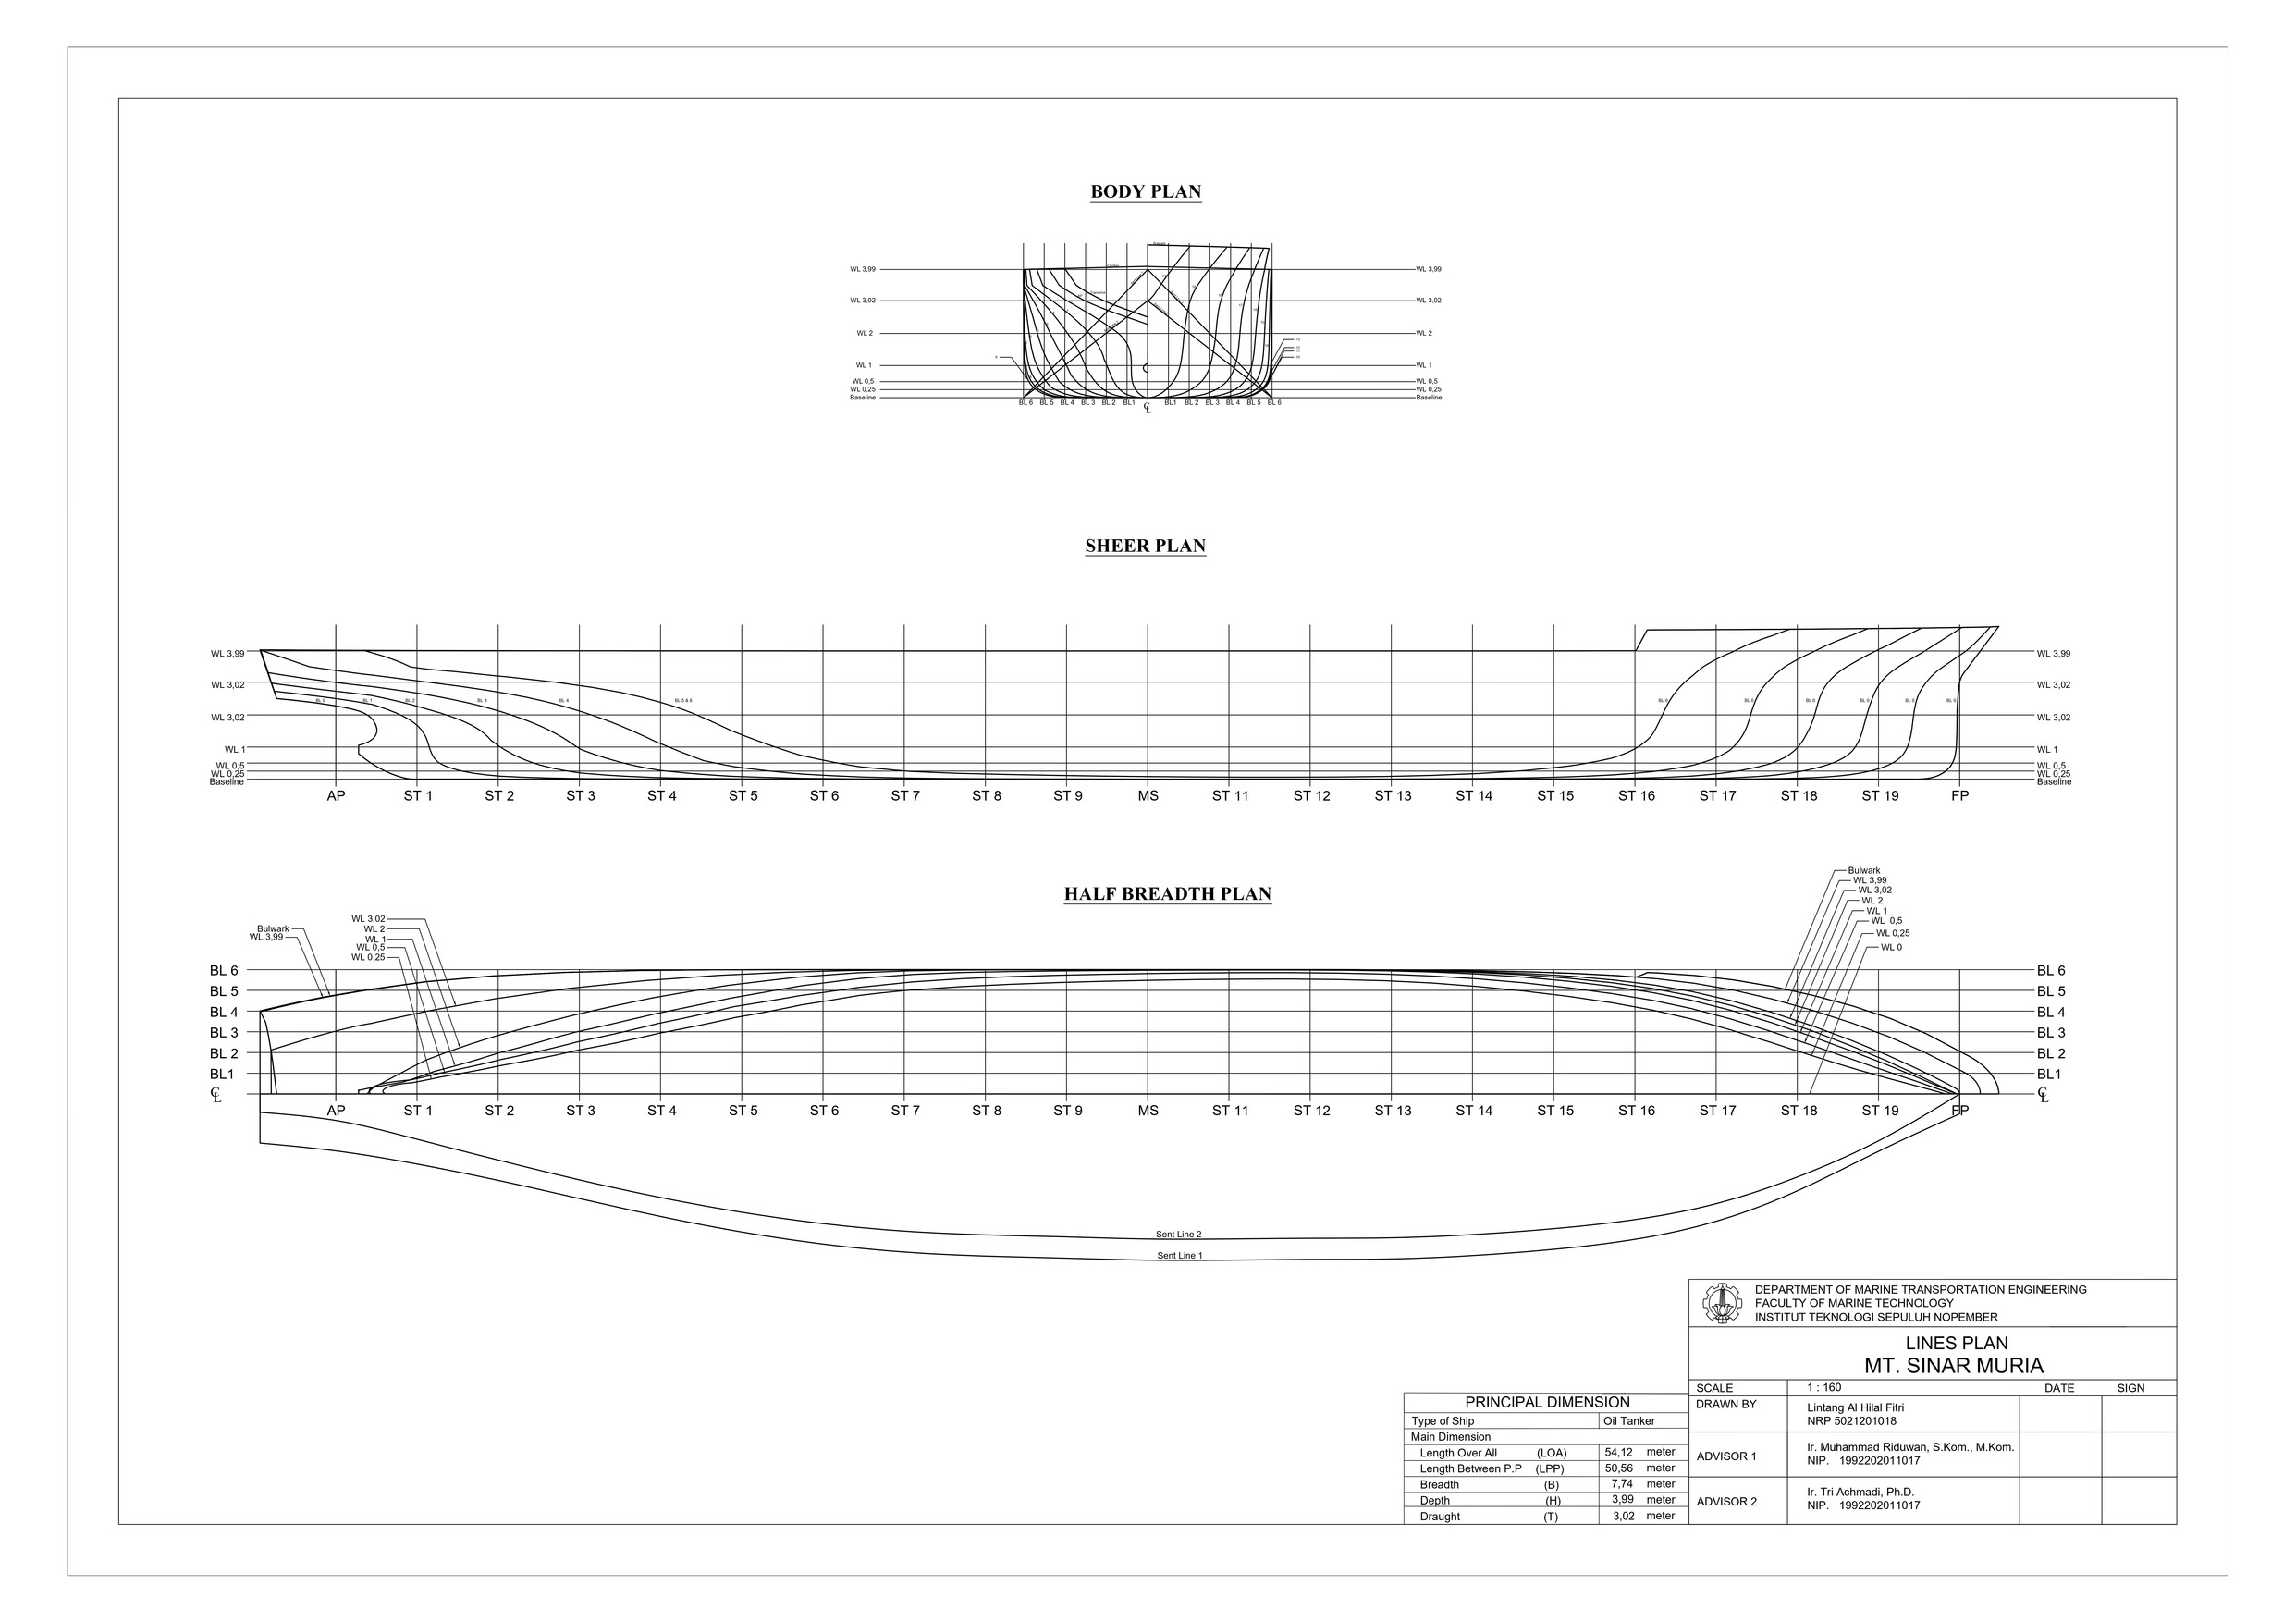
\includegraphics[width=0.9\textwidth]{gambar/Lines Plan 22 Ujil 03 48_page-0001(1).jpg}
    \caption{Rencana Garis Kapal yang Sudah Dibuat}
    \label{fig:lines-plan}
\end{figure}


\subsection{Rencana Umum}
\label{subsec:general-arrangement}

Bentuk lambung yang sudah ada kemudian harus dibagi atau ditentukan penggunaannya dengan tepat. perencanaan ruangan yang dibutuhkan sesuai dengan fungsi dan perlengkapannya ini disebut dengan rencana umum atau \emph{general arrangement} \citep{Taggart_1980}. Beberapa ruangan yang penting diperhatikan adalah ruang muat, kamar mesin dan akomodasi kru kapal. Rencana umum yang dirancang dapat dilihat pada gambar \ref{fig:general-arrangement}

\begin{figure}[htbp!]
    \centering
    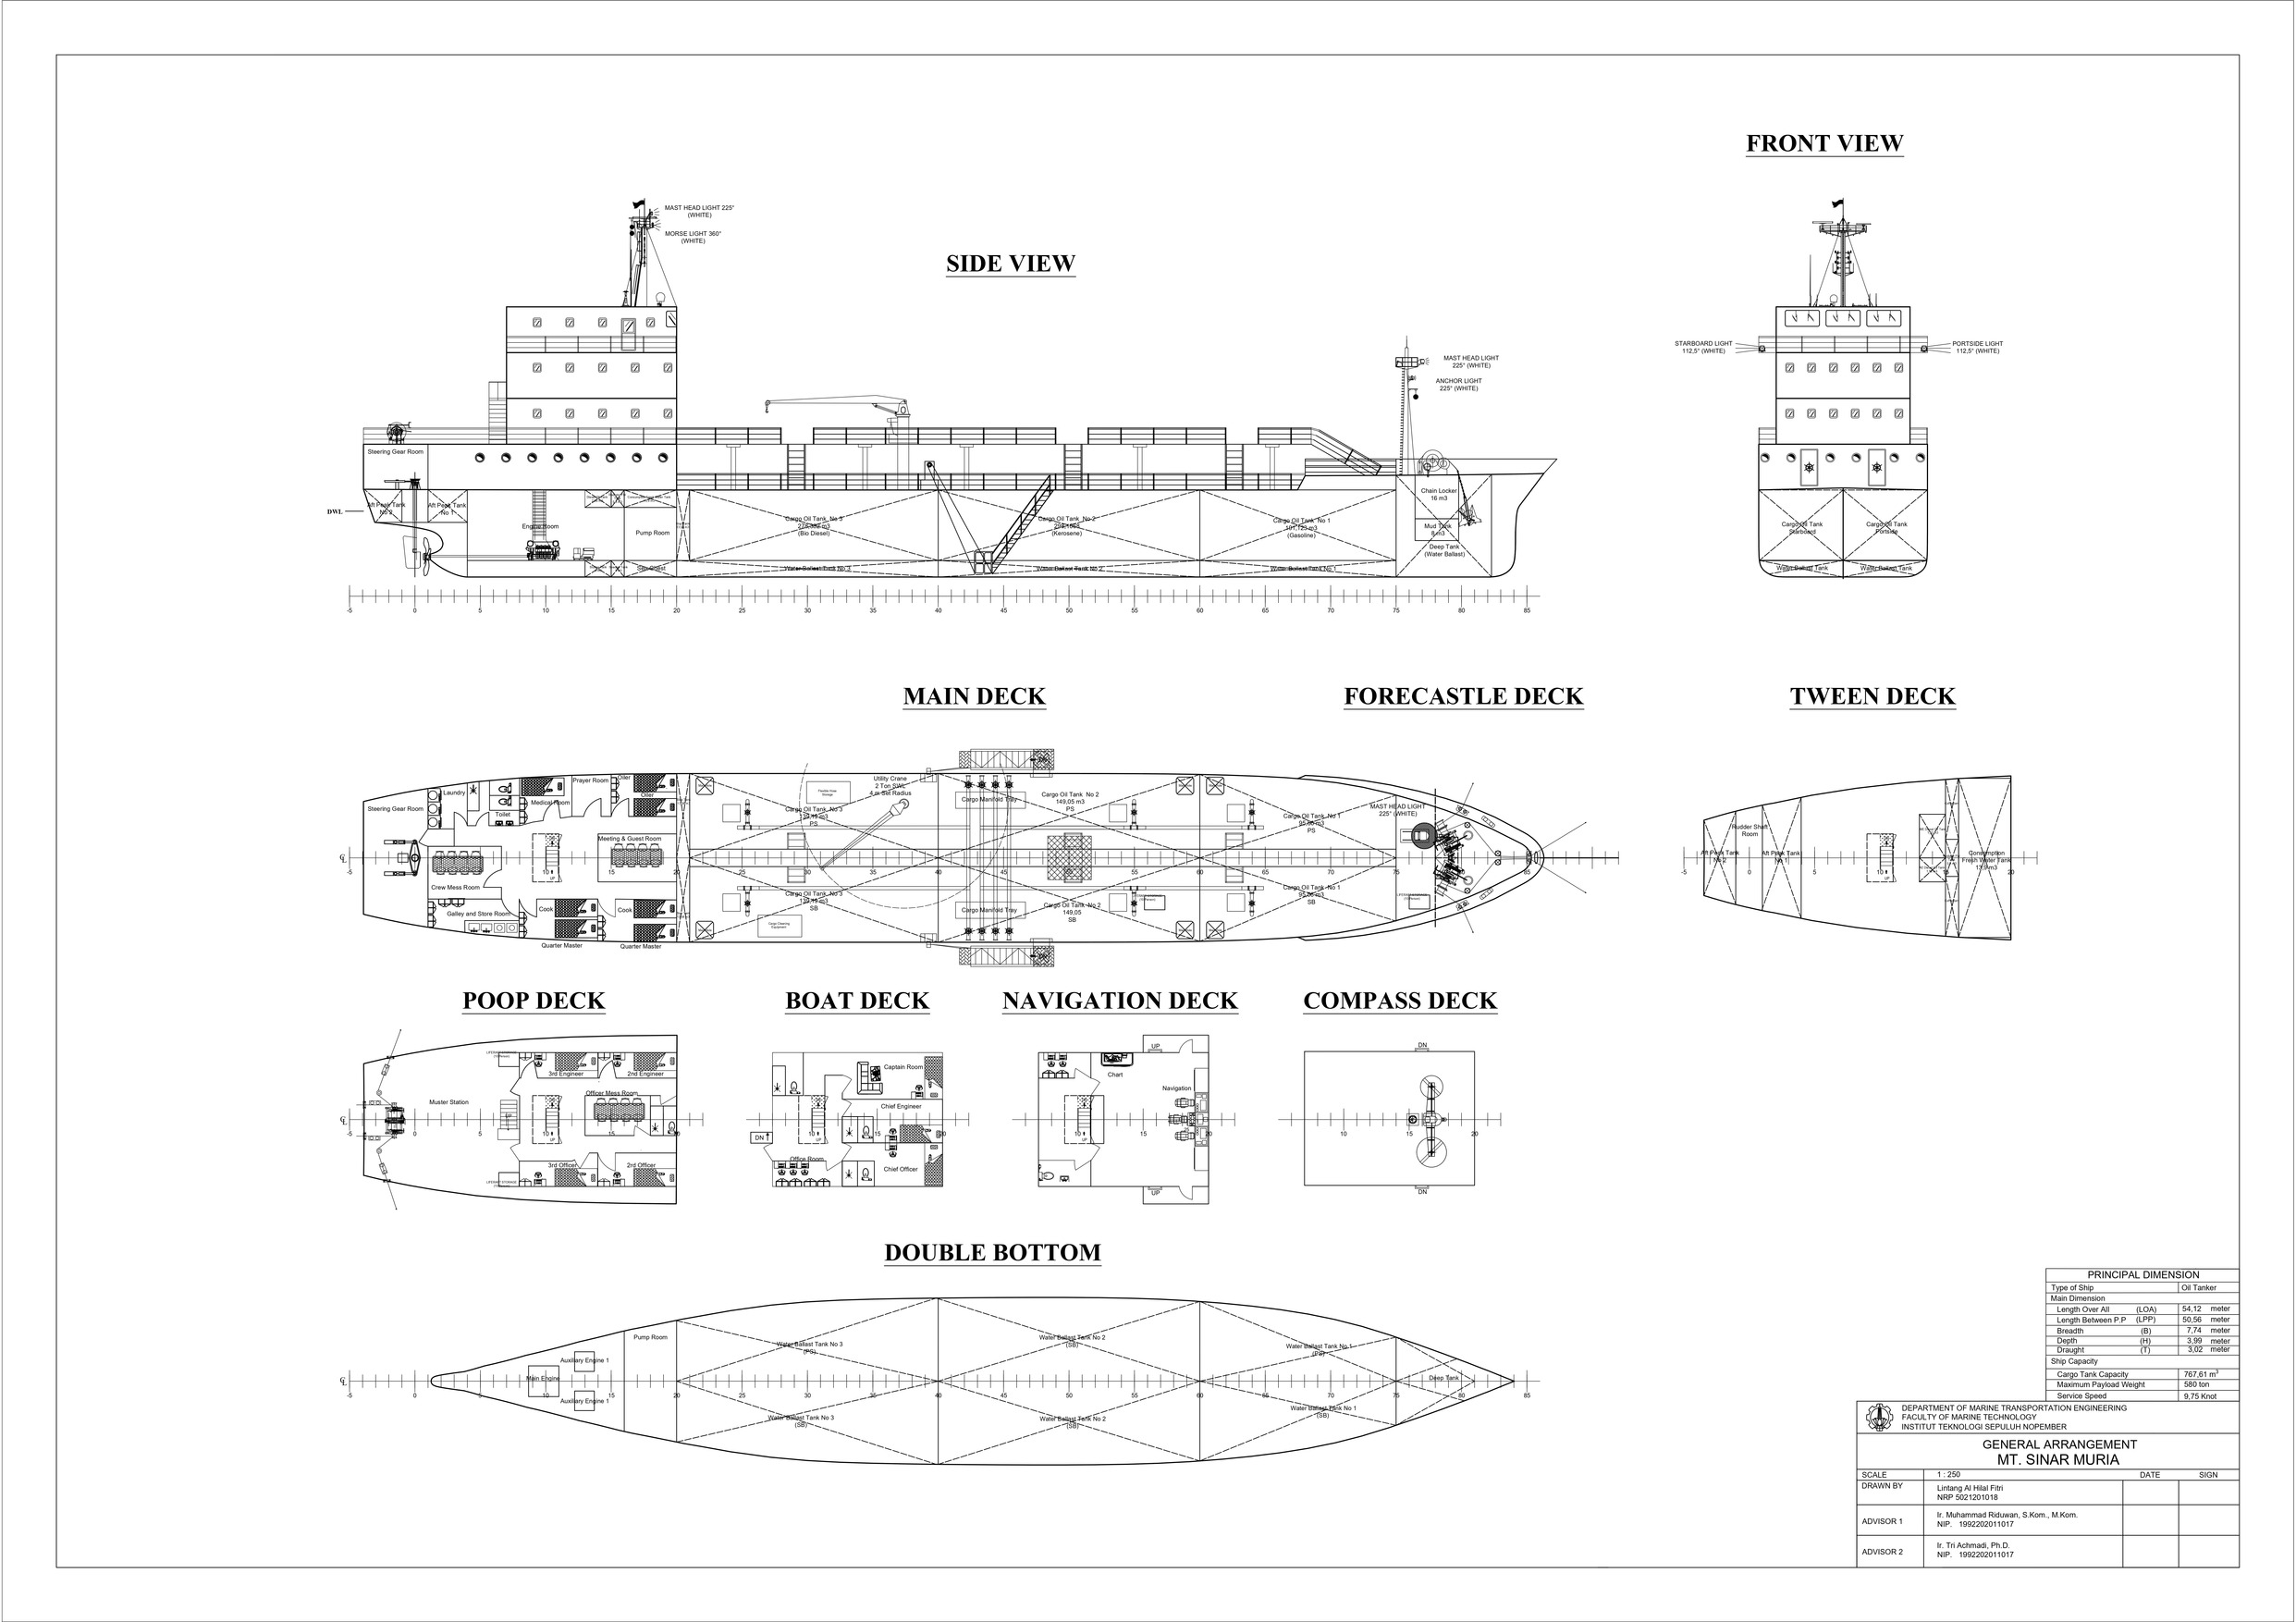
\includegraphics[width=0.9\textwidth]{gambar/GA 22 Juli 03 45_page-0001(1).jpg}
    \caption{Rencana Garis Kapal yang Sudah Dibuat}
    \label{fig:general-arrangement}
\end{figure}

